\documentclass{beamer}

% packages
\usepackage{beamerthemesplit}
\usepackage{enumerate}
\usepackage{amssymb}
\usepackage[all,cmtip]{xy}
\usepackage[mathscr]{eucal}
\usepackage[natbib=true,style=authoryear,backend=bibtex,useprefix=true]{biblatex}
\addbibresource{reading.bib}
\usepackage{graphicx,color}

\title{AlphaFold Bitesized Pieces}
\author{Reuben Brasher}
\date{\today}

\begin{document}

\frame{\titlepage}

\section[Outline]{}
\frame{\tableofcontents}

\section{ML Nutshell}
\frame
{
   \frametitle{How to be an ML Engineer}

   \begin{itemize}
      \item<1-> Define cost function

      \item<2-> Define network architecture
      
      \item<3-> Apply gradient decent
      
   \end{itemize}
}

\frame
{
   \frametitle{Classical Neuralnet}
   
   Refer to Fig. \ref{fig:neuralnet}.
   
   \begin{figure}[ht]
      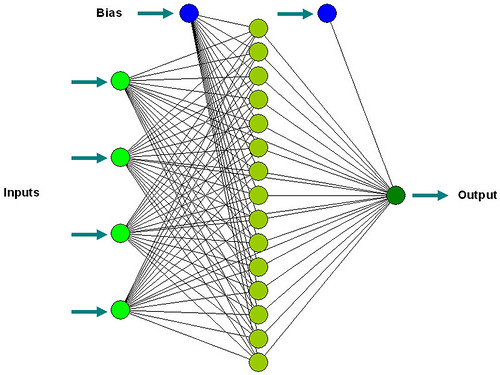
\includegraphics[height=2in,keepaspectratio]{images/7880863848_0698ba4909.jpg}
      \caption{https://search.creativecommons.org/photos/70ab8654-c234-4dbe-9b1c-62851544245a} \label{fig:neuralnet}
   \end{figure}
}

\frame
{
   \frametitle{Dense Layers}

   \begin{itemize}
      \item<1-> Linear function whose coefficients are parameter of model

      \item<2-> Possible non-linear activation function

      \begin{itemize}
         \item tanh
         \item sigmoid or softmax
         \item relu
      \end{itemize}
      
   \end{itemize}
}

\frame
{
   \frametitle{Gate Layers}

   \begin{itemize}
      \item<1-> Entrywise multiplication of two previous layers outputs

      \item<2-> Became popular with LSTM
      
   \end{itemize}
}

\frame
{
   \frametitle{Attention Layers}

   \begin{itemize}
      \item<1-> Define a convex combination along axis of previous layer

      \item<2-> Became popular with
      
   \end{itemize}
}

\frame
{
   \frametitle{Tranformers with Multi-head Attention Layers}

   \begin{itemize}
      \item<1-> Multi-dimensional attention

      \item<2-> Defined in
      
   \end{itemize}
}

\section{Inspiration Papers}

\frame
{
   \frametitle{Human pose estimation with iterative error feedback\cite{carreira2016human}}

   equations
}


\frame
{
   \frametitle{Bert: Pre-training of deep bidirectional transformers for language understanding\cite{devlin2018bert}}

   Model pretrained to reconstruct corrupted text and then finetuned
}



\begin{frame}[t,allowframebreaks]
\frametitle{References}
\printbibliography
\end{frame}

\end{document}
